\documentclass{scrartcl}
        \usepackage{xcolor, tikz}
        \usepackage{pgfplots}
        \pgfplotsset{compat=newest}
        \pagestyle{empty}
        \definecolor{pdg2112}{RGB}{228,26,28}
\definecolor{pdg2212}{RGB}{55,126,184}
\definecolor{pdg1000020040}{RGB}{166,86,40}
\definecolor{pdg11}{RGB}{152,78,163}
\definecolor{pdg1000110230}{RGB}{153,153,153}
\definecolor{pdg22}{RGB}{77,175,74}
\definecolor{pdg1000060120}{RGB}{153,153,153}
\begin{document}
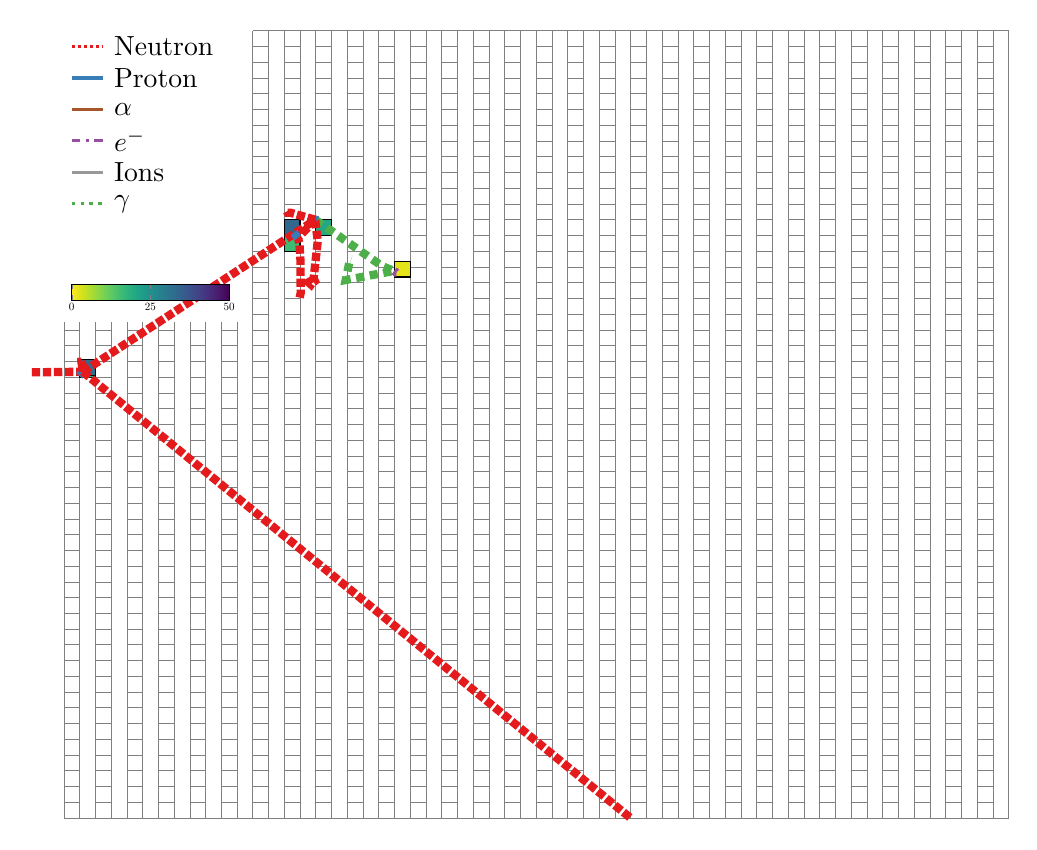
\begin{tikzpicture}[scale=0.4] %\columnwidth/252.0pt]
\draw[step=0.5,very thin,gray] (-0.001000,-12.499) grid (0.500000,3.25);
\draw[step=0.5,very thin,gray] (0.999000,-12.499) grid (1.500000,3.25);
\draw[step=0.5,very thin,gray] (1.999000,-12.499) grid (2.500000,3.25);
\draw[step=0.5,very thin,gray] (2.999000,-12.499) grid (3.500000,3.25);
\draw[step=0.5,very thin,gray] (3.999000,-12.499) grid (4.500000,3.25);
\draw[step=0.5,very thin,gray] (4.999000,-12.499) grid (5.500000,3.25);
\draw[step=0.5,very thin,gray] (5.999000,-12.499) grid (6.500000,12.499);
\draw[step=0.5,very thin,gray] (6.999000,-12.499) grid (7.500000,12.499);
\draw[step=0.5,very thin,gray] (7.999000,-12.499) grid (8.500000,12.499);
\draw[step=0.5,very thin,gray] (8.999000,-12.499) grid (9.500000,12.499);
\draw[step=0.5,very thin,gray] (9.999000,-12.499) grid (10.500000,12.499);
\draw[step=0.5,very thin,gray] (10.999000,-12.499) grid (11.500000,12.499);
\draw[step=0.5,very thin,gray] (11.999000,-12.499) grid (12.500000,12.499);
\draw[step=0.5,very thin,gray] (12.999000,-12.499) grid (13.500000,12.499);
\draw[step=0.5,very thin,gray] (13.999000,-12.499) grid (14.500000,12.499);
\draw[step=0.5,very thin,gray] (14.999000,-12.499) grid (15.500000,12.499);
\draw[step=0.5,very thin,gray] (15.999000,-12.499) grid (16.500000,12.499);
\draw[step=0.5,very thin,gray] (16.999000,-12.499) grid (17.500000,12.499);
\draw[step=0.5,very thin,gray] (17.999000,-12.499) grid (18.500000,12.499);
\draw[step=0.5,very thin,gray] (18.999000,-12.499) grid (19.500000,12.499);
\draw[step=0.5,very thin,gray] (19.999000,-12.499) grid (20.500000,12.499);
\draw[step=0.5,very thin,gray] (20.999000,-12.499) grid (21.500000,12.499);
\draw[step=0.5,very thin,gray] (21.999000,-12.499) grid (22.500000,12.499);
\draw[step=0.5,very thin,gray] (22.999000,-12.499) grid (23.500000,12.499);
\draw[step=0.5,very thin,gray] (23.999000,-12.499) grid (24.500000,12.499);
\draw[step=0.5,very thin,gray] (24.999000,-12.499) grid (25.500000,12.499);
\draw[step=0.5,very thin,gray] (25.999000,-12.499) grid (26.500000,12.499);
\draw[step=0.5,very thin,gray] (26.999000,-12.499) grid (27.500000,12.499);
\draw[step=0.5,very thin,gray] (27.999000,-12.499) grid (28.500000,12.499);
\draw[step=0.5,very thin,gray] (28.999000,-12.499) grid (29.500000,12.499);
\draw[very thin,gray] (0,-12.5) -- (30,-12.5) -- (30,12.5) -- (6,12.5);
\definecolor{tempcolor}{rgb}{0.202219,0.715272,0.476084}\draw[fill=tempcolor,fill opacity=1] (0.500000,1.489412) rectangle (1.000000,1.989412);
\definecolor{tempcolor}{rgb}{0.177423,0.437527,0.557565}\draw[fill=tempcolor,fill opacity=1] (0.500000,1.557958) rectangle (1.000000,2.057958);
\definecolor{tempcolor}{rgb}{0.239374,0.735588,0.455688}\draw[fill=tempcolor,fill opacity=1] (7.000000,5.500000) rectangle (7.500000,6.000000);
\definecolor{tempcolor}{rgb}{0.190631,0.407061,0.556089}\draw[fill=tempcolor,fill opacity=1] (7.000000,6.000000) rectangle (7.500000,6.500000);
\definecolor{tempcolor}{rgb}{0.134692,0.658636,0.517649}\draw[fill=tempcolor,fill opacity=1] (8.000000,6.000000) rectangle (8.500000,6.500000);
\definecolor{tempcolor}{rgb}{0.896320,0.893616,0.096335}\draw[fill=tempcolor,fill opacity=1] (10.500000,4.677954) rectangle (11.000000,5.177954);
\draw[color=pdg2112, line width=3pt, densely dotted] (-1.0152659165562, 1.6506541930040963) -- (-0.015368372371995065, 1.6617324090645265) -- (0.0029999999999745343, 1.6619359187130893) -- (0.48999999999998634, 1.6673315627496303) -- (0.6012055804232432, 1.6685636484310282);
\draw[color=pdg1000020040, line width=3pt, solid] (0.6012055804232432, 1.6685636484310282);
\draw[color=pdg2212, line width=3pt, solid] (0.6012055804232432, 1.6685636484310282) -- (0.581848413530679, 1.6428579102468255) -- (0.573322839508478, 1.6312178164140565) -- (0.5544261456906951, 1.6099386881899904) -- (0.5423751274600818, 1.5949182415944163) -- (0.5330496225205934, 1.5828509329070788) -- (0.5258008202104747, 1.5733714487486934) -- (0.5199055944794736, 1.5657841619771333) -- (0.5154330923786802, 1.5597562276080361) -- (0.5119718719882258, 1.5549795138866902) -- (0.4970000000000027, 1.537107005588512);
\draw[color=pdg2212, line width=3pt, solid] (0.6012055804232432, 1.6685636484310282);
\draw[color=pdg1000020040, line width=3pt, solid] (0.6012055804232432, 1.6685636484310282);
\draw[color=pdg2112, line width=3pt, densely dotted] (0.6012055804232432, 1.6685636484310282) -- (0.9130982446389453, 1.8721898227030322) -- (0.9900000000000319, 1.9223968715874964) -- (1.0935471982188574, 1.9899999999999998) -- (1.1042690450409283, 1.9969999999999999) -- (1.1134591994598622, 2.003) -- (1.1211176614756369, 2.008) -- (1.490000000000009, 2.248833171049781) -- (1.7908281551860454, 2.445235630555765) -- (1.990000000000009, 2.5752694705120662) -- (2.490000000000009, 2.901705769974338) -- (2.6685580657331913, 3.018281438408498) -- (2.9900000000000317, 3.228142069436637) -- (3.3910858029494877, 3.4899999999999998) -- (3.401807649771558, 3.497) -- (3.41099780419047, 3.503) -- (3.418656266206244, 3.5080000000000005) -- (3.490000000000009, 3.554578368898924) -- (3.5462879762802912, 3.591327246261232) -- (3.98515293155383, 3.8778501501875993) -- (4.156932004526311, 3.9900000000000007) -- (4.167653851348382, 3.997) -- (4.176844005767293, 4.003) -- (4.184502467783068, 4.008000000000001) -- (4.490000000000009, 4.207450967823519) -- (4.862882842100953, 4.450895958040333) -- (4.990000000000009, 4.533887267285818) -- (5.490000000000009, 4.86032356674809) -- (5.740612752648076, 5.023941765893066) -- (5.990000000000009, 5.186759866210375) -- (6.454470609256918, 5.489999999999999) -- (6.46519245607899, 5.497) -- (6.474382610497924, 5.503) -- (6.482041072513676, 5.508) -- (6.6183426631951985, 5.596987573745798) -- (6.990000000000009, 5.839632465134943) -- (7.220316810833788, 5.989999999999999) -- (7.2310386576558585, 5.997) -- (7.24022881207477, 6.003) -- (7.2478872740905445, 6.008) -- (7.490000000000009, 6.166068764597228) -- (7.507483062579444, 6.177482977100616) -- (7.934937529015883, 6.456556285524895) -- (7.990000000000009, 6.49250506405952);
\draw[color=pdg1000110230, line width=3pt, solid] (7.991665253975702, 6.493592262750498);
\draw[color=pdg22, line width=3pt, dotted] (7.991665253975702, 6.493592262750498) -- (8.490000000000009, 6.146690121805748) -- (8.990000000000009, 5.798628759727022) -- (9.40462338422633, 5.51) -- (9.423298252247264, 5.497) -- (9.489999999999986, 5.450567397648319) -- (9.990000000000009, 5.102506035569593) -- (10.109640190008236, 5.019221780582332) -- (10.133055386965225, 5.01) -- (10.150829218953026, 5.003) -- (10.166063932085445, 4.997) -- (10.178759526362455, 4.992000000000001) -- (10.488452955904313, 4.870031141046017) -- (10.010000000000014, 4.780123325606878) -- (9.510000000000014, 4.686166527629522) -- (9.010000000000014, 4.592209729652168) -- (8.94995948919593, 4.580927301364016) -- (8.989999999999986, 4.773536116822349) -- (8.992000000000008, 4.783156814040811) -- (8.99699999999998, 4.807208557086796) -- (9.002999999999997, 4.836070648742121) -- (9.007999999999992, 4.860122391788154) -- (9.010000000000014, 4.869743089006586) -- (9.034999624925991, 4.99) -- (9.088832238939336, 5.2489536399489225) -- (9.12678838414331, 5.2372262900649895);
\draw[color=pdg11, line width=3pt, dashdotted] (10.488452955904313, 4.870031141046017) -- (10.534822602995996, 4.83483651776987) -- (10.548682775805968, 4.819006671848626) -- (10.56393265459958, 4.818492903546113);
\draw[color=pdg11, line width=3pt, dashdotted] (10.109640190008236, 5.019221780582332);
\draw[color=pdg2212, line width=3pt, solid] (7.991665253975702, 6.493592262750498);
\draw[color=pdg2112, line width=3pt, densely dotted] (7.991665253975702, 6.493592262750498) -- (7.509999999999991, 6.629137758711425) -- (7.204767103028712, 6.715033396941647) -- (7.103758391030192, 6.717068004550159) -- (7.074310300961429, 6.771991365887844);
\draw[color=pdg2212, line width=3pt, solid] (7.074310300961429, 6.771991365887844);
\draw[color=pdg2112, line width=3pt, densely dotted] (7.991665253975702, 6.493592262750498) -- (7.992000000000007, 6.479784118434809) -- (7.992844195454109, 6.444961381748636) -- (7.992000000000007, 6.434038565532573) -- (7.989999999999986, 6.408161107503325) -- (7.992000000000007, 6.388583984979229) -- (7.99699999999998, 6.348147513981212) -- (8.002999999999997, 6.299623748783356) -- (8.007999999999992, 6.259187277785258) -- (8.010000000000014, 6.243012689385981) -- (8.038812193996478, 6.01) -- (8.062871467385047, 5.815425577877599) -- (8.028907193363171, 5.51) -- (8.010000000000014, 5.339976037313145) -- (8.007999999999992, 5.321990928743906) -- (8.002999999999997, 5.2770281573211735) -- (7.9970000000000026, 5.223072831613839) -- (7.992000000000007, 5.178110060191017) -- (7.989999999999986, 5.160124951621834) -- (7.965829896736477, 4.942773985961327) -- (7.931763761026377, 4.636432411322801) -- (7.971053621541477, 4.548834139115587) -- (7.867386119420462, 4.468067431554665) -- (7.848329572906778, 4.439509922923165) -- (7.701292570382316, 4.570959415067682) -- (7.671750172141833, 4.623744346552674) -- (7.659965820555863, 4.639088788783651);
\draw[color=pdg2212, line width=3pt, solid] (7.971053621541477, 4.548834139115587);
\draw[color=pdg2212, line width=3pt, solid] (7.931763761026377, 4.636432411322801);
\draw[color=pdg2212, line width=3pt, solid] (7.991665253975702, 6.493592262750498) -- (8.028905798216261, 6.485064717831058) -- (8.04414741064993, 6.481553719252031) -- (8.056316485264869, 6.478711532445741) -- (8.06601851387354, 6.476170747647243);
\draw[color=pdg2112, line width=3pt, densely dotted] (7.991665253975702, 6.493592262750498) -- (7.990000000000009, 6.491899316534583) -- (7.9410147143775704, 6.442099433069311) -- (7.882845174662544, 6.3829625665138305) -- (7.824675634947539, 6.32382569995835) -- (7.766506095232512, 6.264688833402869) -- (7.708336555517508, 6.205551966847389) -- (7.650167015802481, 6.146415100291907) -- (7.591997476087454, 6.087278233736427) -- (7.533827936372449, 6.028141367180948) -- (7.509999999999968, 6.003917185582575) -- (7.507999999999993, 6.001883926703629) -- (7.5029999999999974, 5.9968007795062075) -- (7.4970000000000026, 5.990701002869298) -- (7.491999999999985, 5.985617855671867) -- (7.489999999999986, 5.983584596792905) -- (7.428506090570318, 5.921068078117765) -- (7.480119353317059, 5.7589818166532245) -- (7.489999999999986, 5.598219372725469) -- (7.492000000000007, 5.565678497803484) -- (7.495852293335952, 5.503) -- (7.4970000000000026, 5.484326310499056) -- (7.5029999999999974, 5.386703685733852) -- (7.507999999999993, 5.305351498429431) -- (7.510000000000014, 5.2728106235075485) -- (7.516490081916572, 5.167214151568186) -- (7.5204482055776225, 4.167183220469747) -- (7.510000000000014, 4.117405981915709) -- (7.507999999999993, 4.107877601528392) -- (7.50300000000002, 4.084056650560255) -- (7.4970000000000026, 4.055471509398348) -- (7.492000000000007, 4.031650558430163) -- (7.489999999999986, 4.022122178042876);
\draw[color=pdg2212, line width=3pt, solid] (7.428506090570318, 5.921068078117765) -- (7.4014777909960685, 5.956036299970515) -- (7.38015193318854, 5.984288525600012) -- (7.375632962146301, 5.99) -- (7.370046206334564, 5.997) -- (7.365190577641897, 6.003) -- (7.361144220398001, 6.008) -- (7.346528874060323, 6.029281429678945) -- (7.3368129250120315, 6.044477552108122) -- (7.328622065820445, 6.057058967072697) -- (7.32196262600562, 6.066739719941717) -- (7.316671475433123, 6.0743697378078405) -- (7.312589255769899, 6.080255831607549) -- (7.309212683107671, 6.0846024365670885);
\draw[color=pdg2112, line width=3pt, densely dotted] (0.6012055804232432, 1.6685636484310282) -- (0.5956528644208674, 1.7067852139238056) -- (0.5926459223615211, 1.7310791235969898) -- (0.5581586257849039, 2.009711452178858) -- (0.5644165719892044, 1.9900270118580807) -- (0.5581620173435112, 1.9893499009169655) -- (0.5610873701854189, 1.9296392207139506);
\draw[color=pdg2212, line width=3pt, solid] (0.5581620173435112, 1.9893499009169655);
\draw[color=pdg2212, line width=3pt, solid] (0.5644165719892044, 1.9900270118580807);
\draw[color=pdg1000060120, line width=3pt, solid] (0.5581586257849039, 2.009711452178858);
\draw[color=pdg2112, line width=3pt, densely dotted] (0.6012055804232432, 1.6685636484310282) -- (0.9899999999999863, 1.3518201777801866) -- (1.4095754291211962, 1.0100000000000002) -- (1.490000000000009, 0.9444796210462794) -- (1.9899999999999864, 0.5371390643124219) -- (2.023312499656322, 0.51) -- (2.4899999999999864, 0.12979850757851893) -- (2.9899999999999864, -0.2775420491553572) -- (3.2507866407265738, -0.49000000000000005) -- (3.4899999999999864, -0.684882605889247) -- (3.9899999999999864, -1.0922231626231231) -- (4.478260781796825, -1.49) -- (4.989999999999986, -1.9069042760908725) -- (5.091997852331952, -1.9899999999999998) -- (5.490000000000009, -2.314244832824774) -- (5.989999999999986, -2.721585389558631) -- (6.319471993402203, -2.99) -- (6.490000000000009, -3.1289259462925396) -- (6.957490901546294, -3.509781954500302) -- (6.991999999999985, -3.537895865253329) -- (7.489999999999986, -3.9436070597602844) -- (7.989999999999986, -4.350947616494161) -- (8.160683205007604, -4.49) -- (8.489999999999986, -4.758288173228047) -- (8.989999999999986, -5.1656287299619255) -- (9.388157346077856, -5.489999999999999) -- (9.489999999999986, -5.572969286695814) -- (9.989999999999986, -5.9803098434296915) -- (10.490000000000009, -6.387650400163594) -- (10.989999999999986, -6.794990956897452) -- (11.22936855768321, -6.990000000000002) -- (11.490000000000009, -7.20233151363136) -- (11.989999999999986, -7.6096720703652165) -- (12.456842698753462, -7.99) -- (12.490000000000009, -8.017012627099126) -- (12.989999999999986, -8.424353183832983) -- (13.070579769288589, -8.49) -- (13.489999999999986, -8.831693740566887) -- (13.989999999999963, -9.239034297300764) -- (14.298053910358794, -9.489999999999998) -- (14.490000000000009, -9.646374854034653) -- (14.989999999999963, -10.053715410768513) -- (15.490000000000009, -10.461055967502427) -- (15.901436025024964, -10.7962451264905) -- (15.937211805518904, -10.825390979178461) -- (15.99699999999998, -10.874099292030541) -- (16.13926512196424, -10.99) -- (16.489999999999963, -11.275737080970123) -- (16.99000000000001, -11.683077637704036) -- (17.366739263034514, -11.99) -- (17.489999999999963, -12.09041819443787) -- (17.99000000000001, -12.497758751171784);
\draw[color=pdg2112, very thick, densely dotted] (0.25,12) -- (1.25,12) node [right,black] {Neutron};
\draw[color=pdg2212, very thick, solid] (0.25,11) -- (1.25,11) node [right,black] {Proton};
\draw[color=pdg1000020040, very thick, solid] (0.25,10) -- (1.25,10) node [right,black] {$\alpha$};
\draw[color=pdg11, very thick, dashdotted] (0.25,9) -- (1.25,9) node [right,black] {$e^-$};
\draw[color=pdg1000110230, very thick, solid] (0.25,8) -- (1.25,8) node [right,black] {Ions};
\draw[color=pdg22, very thick, dotted] (0.25,7) -- (1.25,7) node [right,black] {$\gamma$};

        \begin{axis}[%
            at={(0.25cm,4.75cm)},
            hide axis,
            scale only axis,
            height=0pt,
            width=0pt,
            colormap={reverse viridis}{
                indices of colormap={
                \pgfplotscolormaplastindexof{viridis},...,0 of viridis}
            },
            colorbar horizontal,
            point meta min=0,
            point meta max=50,
            colorbar style={
                width=5cm,
                xtick={50, 25, 0},
            }]
        \end{axis}
        
        \end{tikzpicture}
        \end{document}
        